\documentclass[11pt,UTF8]{article}
\usepackage[no-math,cm-default]{fontspec}
\usepackage{amsmath}
\usepackage{amsthm}
\usepackage{amssymb}
\usepackage{xeCJK}
\usepackage{verbatim}
\usepackage{indentfirst}
\usepackage{syntonly}
\usepackage{fancyhdr}
\usepackage[unicode=true, colorlinks, linkcolor=black, anchorcolor=black, citecolor=black, urlcolor=black]{hyperref}
\usepackage{graphicx}
\usepackage[top = 1.2in, bottom = 1.2in, left = 1.3in, right = 1.3in]{geometry}
\usepackage{xcolor}
\usepackage{paralist}
\usepackage{ulem}
\usepackage{titlesec}
\usepackage{zhspacing}
\usepackage{booktabs}
\usepackage{multirow}
\usepackage{supertabular}
\usepackage{float}
\usepackage{soul}
\usepackage{longtable}
\usepackage{listings}
\usepackage{xcolor}
\usepackage{multicol}
\lstset{
    numbers=left, 
    numberstyle= \tiny, 
    keywordstyle= \color{ blue!70},
    commentstyle= \color{red!50!green!50!blue!50}, 
    frame=shadowbox, % 阴影效果
    rulesepcolor= \color{ red!20!green!20!blue!20} ,
    escapeinside=``, % 英文分号中可写入中文
    xleftmargin=2em,xrightmargin=2em, aboveskip=1em,
    framexleftmargin=2em
} 

\defaultfontfeatures{Mapping=tex-text}
%\setromanfont{Times New Roman}
%\newfontfamily\zhfont[BoldFont=Adobe Heiti Std]{Adobe Song Std}
\setmonofont[Scale=1]{Courier New}
\XeTeXlinebreaklocale "zh"
\XeTeXlinebreakskip = 0pt plus 1pt

\definecolor{hlcolor}{rgb}{0.9, 0.9, 0.9}
\sethlcolor{hlcolor}
\newcommand{\code}[1]{\texttt{\hl{#1}}}

\newcommand{\hlink}[1]{
	\footnote{\href{#1}{\textsl{\underline{#1}}}}
}
\renewenvironment{proof}{\noindent{\textbf{证明:}}}{\hfill $\square$ \vskip 4mm}
\newtheorem{conclusion*}{结论}
\newcommand{\conclusion}[1]{
	\begin{conclusion*}\textup{#1}\end{conclusion*}
}
\let\enumerate\compactenum
\let\endenumerate\endcompactenum
\let\itemize\compactitem
\let\enditemize\endcompactitem
\setlength{\pltopsep}{5pt}
\setlength{\parindent}{2em}
\setlength{\footskip}{30pt}
\setlength{\baselineskip}{1.3\baselineskip}
\renewcommand\arraystretch{1.2}

\lstset{language=C++,
	backgroundcolor=\color{hlcolor},
	extendedchars=false,
	basicstyle=\ttfamily,
	keywordstyle=\bfseries,
	commentstyle=\itshape\color{gray},
	escapeinside=`'}

\title{\fontsize{25pt}{\baselineskip}\textbf{图形学第四次作业\\[2ex]实验报告}}
\author{1600012938~周尚彦}
%\date{}

\pagestyle{fancy}
\renewcommand{\sectionmark}[1]{\markright{\thesection.\ #1}}
\renewcommand{\subsectionmark}[1]{}
%\fancyhead[C]{\small 湖南师大附中}
\fancyhead[L]{\small\slshape 图形学第四次作业}
\fancyhead[R]{\small\slshape\nouppercase{\rightmark}}
\fancypagestyle{plain}{\fancyhead{}\fancyfoot{}\renewcommand{\headrulewidth}{0pt}}

%\titleformat*{\section}{\fontsize{16pt}{\baselineskip}\bfseries}




\newcommand{\graph}[2]
{
\begin{figure}[H]
	\centering
	\includegraphics[width=\textwidth]{#1}
	\caption{#2}
\end{figure}
}

\begin{document}

\thispagestyle{plain}

\maketitle

%\setcounter{tocdepth}{1}
%\renewcommand{\contentsname}{\LARGE 目录}
\tableofcontents

\pagenumbering{arabic}
\setcounter{section}{0}

\section{代码与运行环境}
	\begin{itemize}
		\item 代码均在windows10 64位系统环境下使用visual studio 2017编译运行。
		\item 使用的第三方库有GLFW,GLEW,GLM,SOIL。
	\end{itemize}
\newpage

\section{凹凸纹理贴图 Normal Mapping}
\subsection{算法流程}
	\begin{enumerate}
		\item 从法线纹理图中读取纹理
		\item 使用Mipmap为每个片段获取法向量
		\item 使用Blinn算法利用从纹理中获取的法向量计算光照
	\end{enumerate}

\subsection{实验结果}
	\begin{figure}[H]
		\centering
		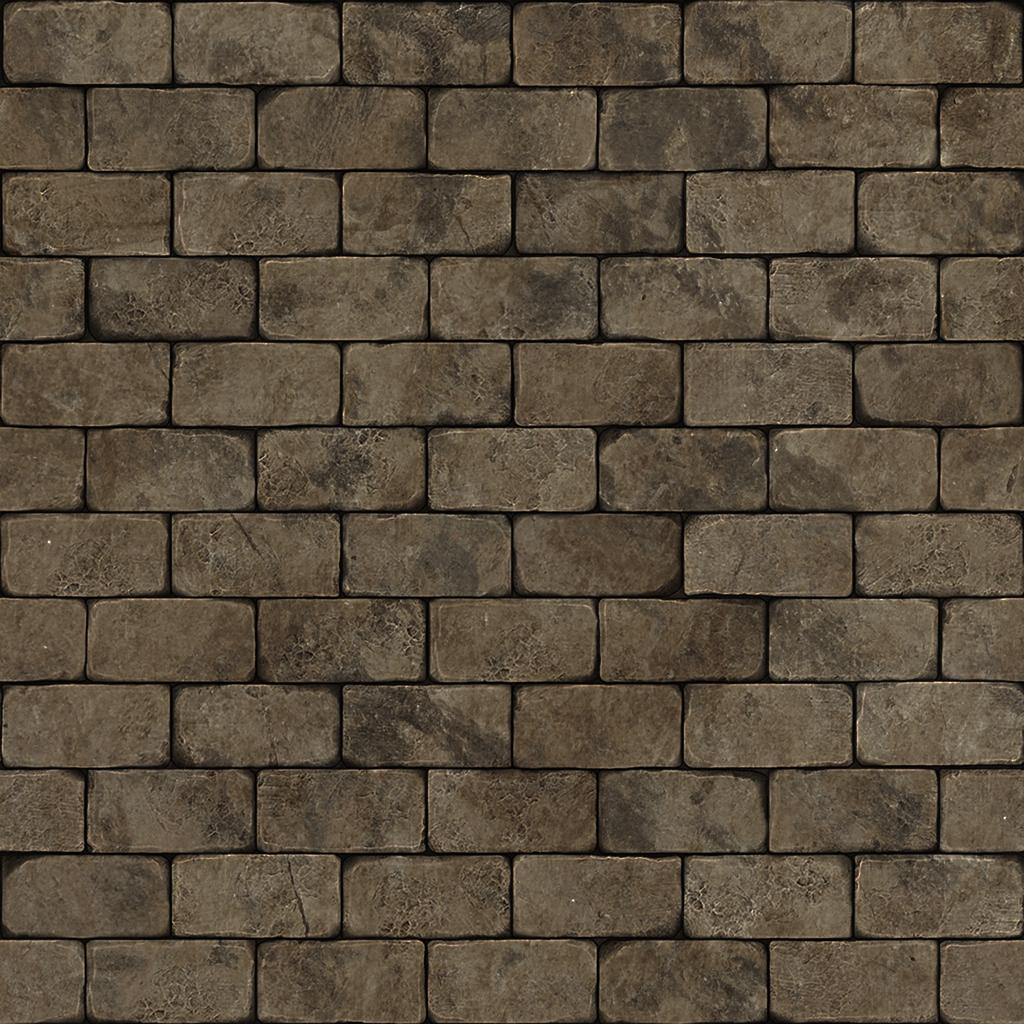
\includegraphics[width=\textwidth]{brickwall.jpg}
		\caption{原图}\label{original}
	\end{figure}

	\begin{figure}[H]
		\centering
		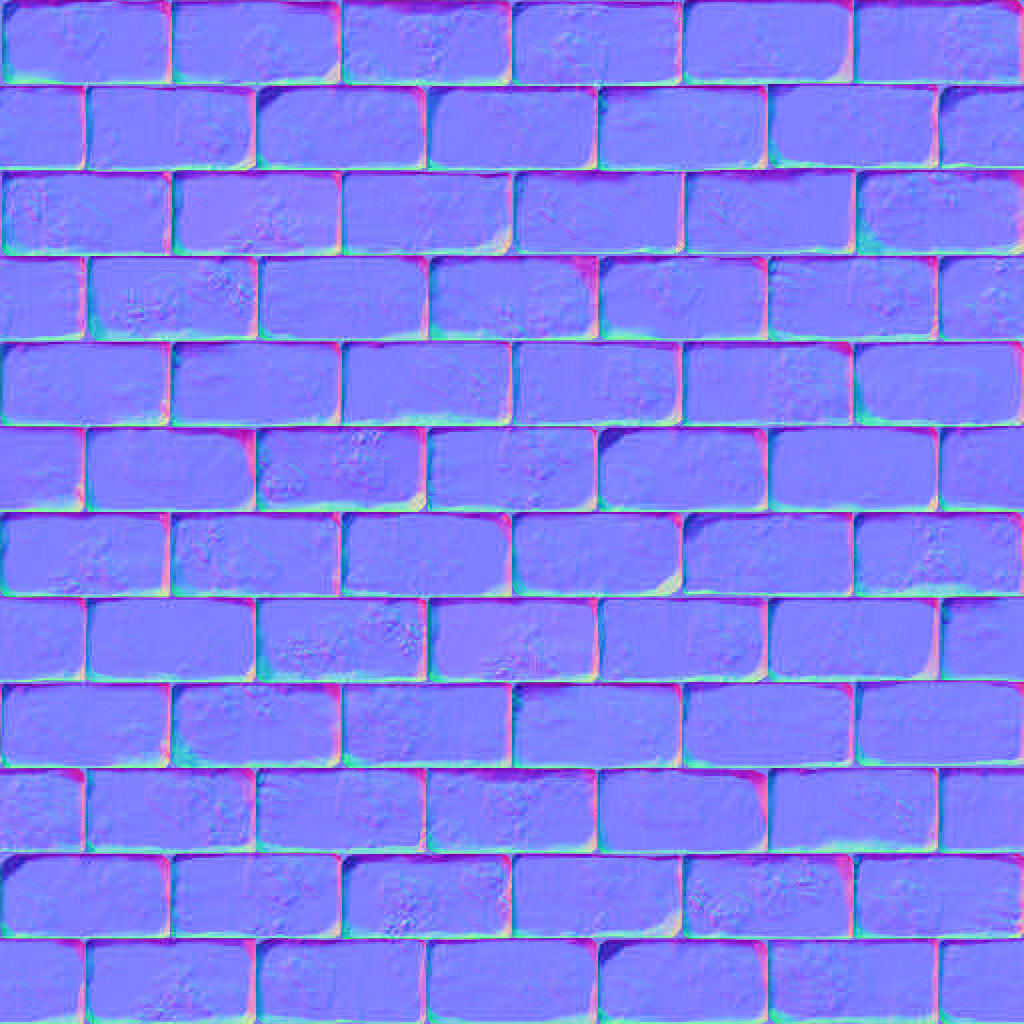
\includegraphics[width=\textwidth]{brickwall_normal.jpg}
		\caption{法线纹理图}\label{normal}
	\end{figure}	

	\begin{figure}[H]
		\centering
		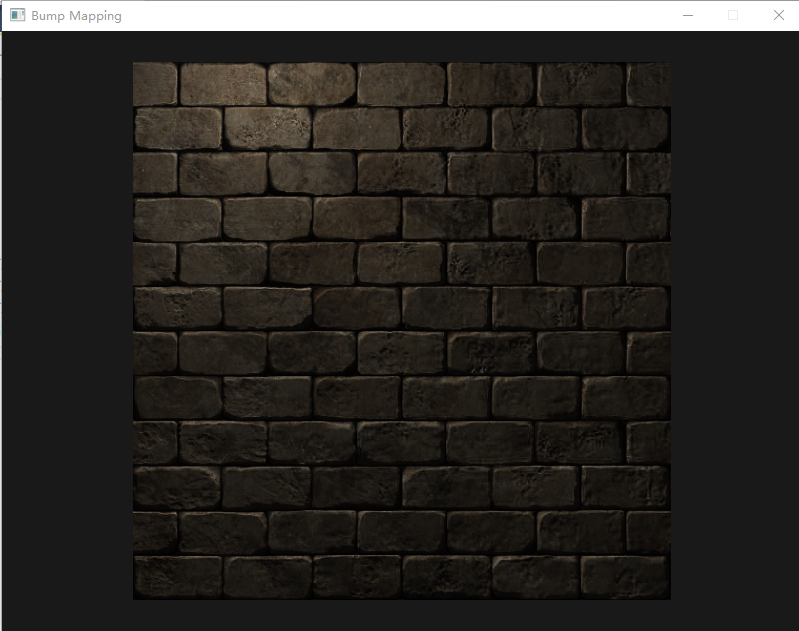
\includegraphics[width=\textwidth]{result.png}
		\caption{实验结果}\label{result}
	\end{figure}

\newpage
\end{document}
